%%%%%%%%%%%%%%%%%%%%%%%%%%%%%%%%%%%%%%%%%%%%%%%%%%%%%%%%%%%%%%%%%%%%%%%%%%
% Copyright (c) 2011, ETH Zurich.
% All rights reserved.
%
% This file is distributed under the terms in the attached LICENSE file.
% If you do not find this file, copies can be found by writing to:
% ETH Zurich D-INFK, Haldeneggsteig 4, CH-8092 Zurich. Attn: Systems Group.
%%%%%%%%%%%%%%%%%%%%%%%%%%%%%%%%%%%%%%%%%%%%%%%%%%%%%%%%%%%%%%%%%%%%%%%%%%

\documentclass[a4paper,twoside]{report} % for a report (default)

\usepackage{bftn,color} % You need this
\usepackage{subfig}
\usepackage{listings}
\usepackage{verbatim}

\title{Barrelfish Architecture Overview}   % title of report
\author{Team Barrelfish}	% author
\tnnumber{000}  % give the number of the tech report
\tnkey{Barrelfish Overview} % Short title, will appear in footer

% \date{Month Year} % Not needed - will be taken from version history

%% \newcommand{\note}[1]{}
\newcommand{\note}[1]{[\textcolor{red}{\textit{#1}}]}

\begin{document}
\maketitle

%
% Include version history first
%
\begin{versionhistory}
\vhEntry{1.0}{24.06.2010}{ikuz, amarp}{Initial version}
\end{versionhistory}

% \intro{Abstract}		% Insert abstract here
% \intro{Acknowledgements}	% Uncomment (if needed) for acknowledgements
% \tableofcontents		% Uncomment (if needed) for final draft
% \listoffigures		% Uncomment (if needed) for final draft
% \listoftables			% Uncomment (if needed) for final draft



%%%%%%%%%%%%%%%%%%%%%%%%%%%%%%%%%%%%%%%%%%%%%%%%%%%%%%%%%%%%%%%%%%%%%%%%%%%%%%%%
\chapter{Barrelfish Architecture Overview}

We start with a high level overview of the architecture of the Barrelfish
Operating System.

\section{High level Architecture Overview}\label{sec:overview}
Figure~\ref{fig:os-arch} shows an overview of the components of the OS.  Each
core runs a kernel which is called a "CPU driver". The CPU driver maintains
capabilities, executes syscalls on capabilities, schedules dispatchers, and
processes interrupts, pagefaults, traps, and exceptions.

The kernel schedules and runs "Dispatchers". Dispatchers are an implementation
of scheduler activations, thus each dispatcher can run and schedule its own
threads.  Multiple dispatchers can be combined into a domain. Typically this is
used to combine related dispatchers running on different cores. Often
dispatchers in a domain share (all or part of) their vspace. Unless dispatchers
in a domain run on the same core (which is possible, but rare) they cannot share
a cspace (since cspaces are core specific).

Typically we refer to user level processes (or services or servers) as "user
domains". Often these consist of single dispatchers running on a single core.

\begin{figure}[hbt]
 \begin{center}
 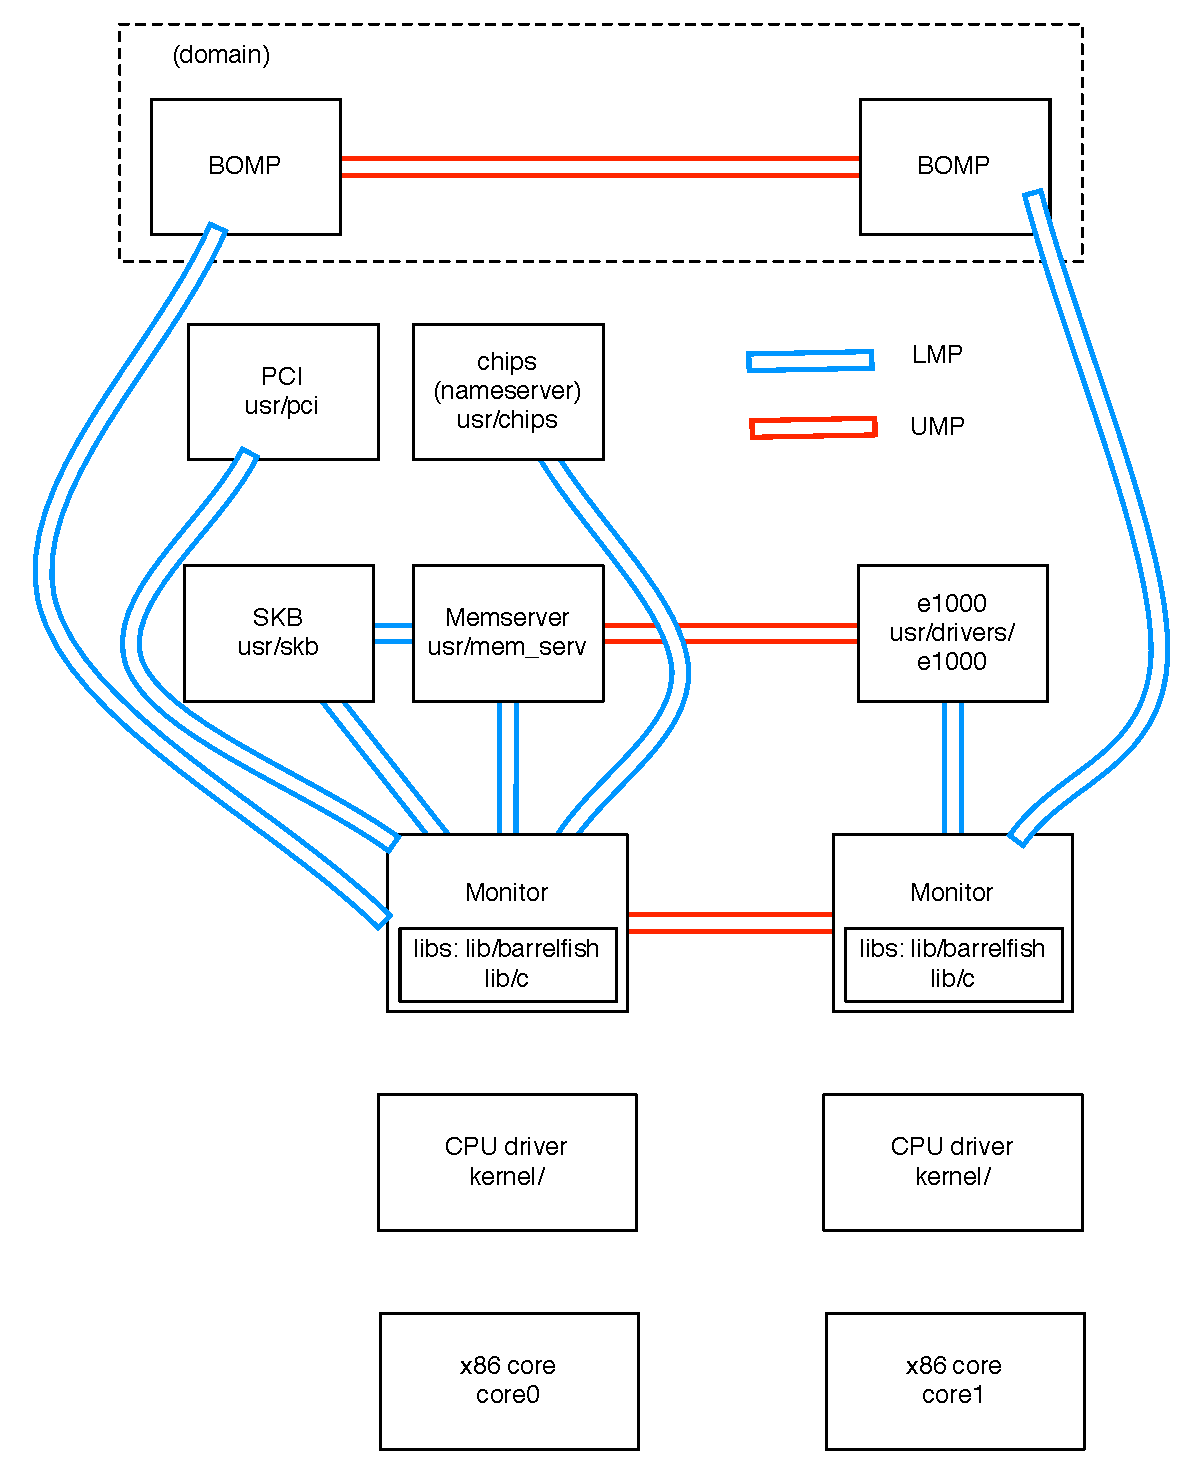
\includegraphics[width=0.5\columnwidth]{os-arch.pdf}
 \end{center}
 \caption{High level overview of the Barrelfish OS architecture}\label{fig:os-arch}
\end{figure}


\section{Dispatcher}
The dispatcher is unit of kernel scheduling, and it is responsible for managing
its own threads.

\begin{figure}[hbt]
 \begin{center}
 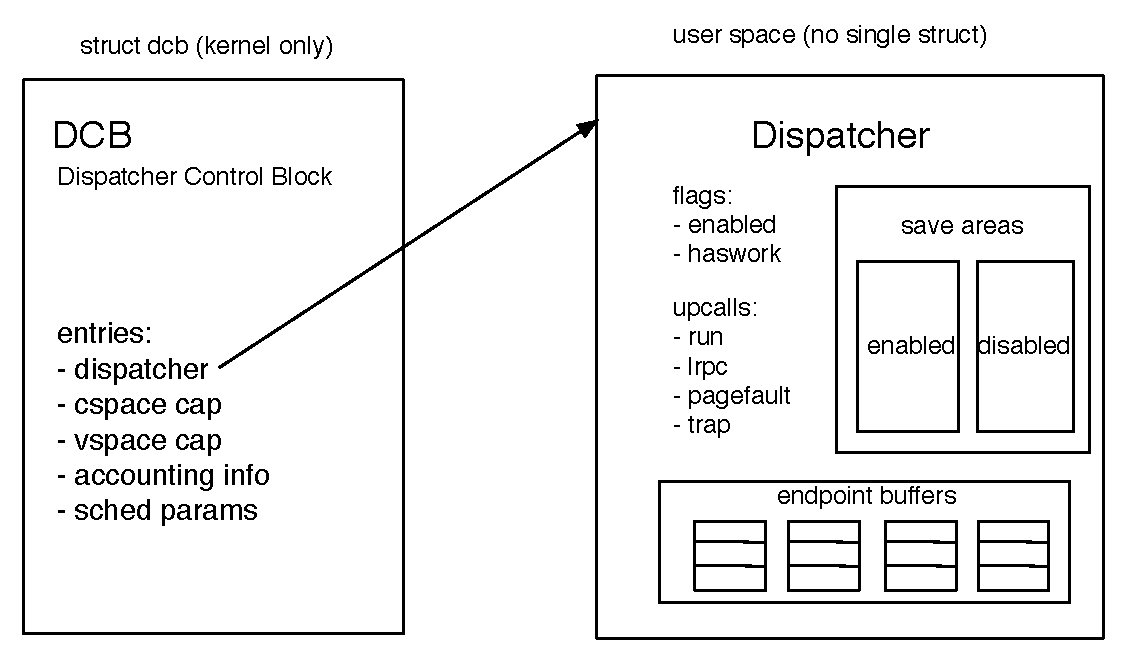
\includegraphics[width=0.5\columnwidth]{dcb.pdf}
 \end{center}
 \caption{Dispatcher Control Block}\label{fig:dcb}
\end{figure}

The kernel maintains a DCB (dispatcher control block) for each dispatcher
(Figure~\ref{fig:dcb}). The DCB contains entries that define the dispatcher's
cspace (capability tables), vspace (page tables), some scheduling parameters,
and a pointer to a user space dispatcher structure (actually it consists of
several structs). This struct manages the scheduling of the dispatcher's
threads.

The dispatcher can be in one of two modes: enabled and disabled. It is in
enabled mode when running user thread code. It is in disabled mode when running
dispatcher code (e.g., when managing TCBs, run queues, etc.). The dispatcher
defines a number of upcall entry points that are invoked by the kernel when it
schedules the dispatcher.

The main upcall is \texttt{run()}.  When the kernel decides to schedule a
dispatcher, it brings in the base page table pointed to by the vspace
capability, and calls the dispatcher's \texttt{run()} upcall.  The dispatcher
must decide which thread it wants to run, restore the thread's state, and then
run it. Note that when \texttt{run()} is invoked the dispatcher first runs in
disabled mode until the thread actually starts executing at which point the
dispatcher switches to enabled mode.

When a dispatcher running in enabled mode is preempted, the kernel saves all
register state to a save area (labelled "enabled"). When the dispatcher is next
restarted it can restore this register state and run the preempted thread, or it
can decide to schedule another thread, in which case it must first save the
saved registers to a TCB.  

When the kernel preempts a dispatcher running in disabled state, it stores the
register state in a save area labelled "disabled". When the kernel schedules a
dispatcher that is in disabled state, it does not invoke \texttt{run()}. Instead
it restores the registers stored in the disabled save area. This causes the
dispatcher to resume execution from where it was preempted.

\section{Capabilities}

The Barrelfish capability model is similar to the seL4 model. Kernel objects are
referenced by partitioned capabilities. The actual capability can only be
directly accessed and manipulated by the kernel, while user level only has
access to capability references (\texttt{struct capref}), which are addresses in
a cspace. User level can only manipulate capabilities using kernel system calls
(to which it passes capability references). In processing a system call the
kernel looks up the capability reference in the appropriate cspace to find the
actual capability; this process is similar to the translation of a virtual
address to a physical address (Figure~\ref{fig:cap_translation}). A capability
reference can be used to get \texttt{caddr\_t} and \texttt{valid bits} which are
used in system calls (see \texttt{include/barrelfish/caddr.h}).  Valid bits are
used when the user wants to access cnode type capabilities (else, the
translation process would continue by looking at entries in the cnode).

 
\begin{figure}
  \centering
  \subfloat[capref to capability translation.]{\label{fig:cap_translation}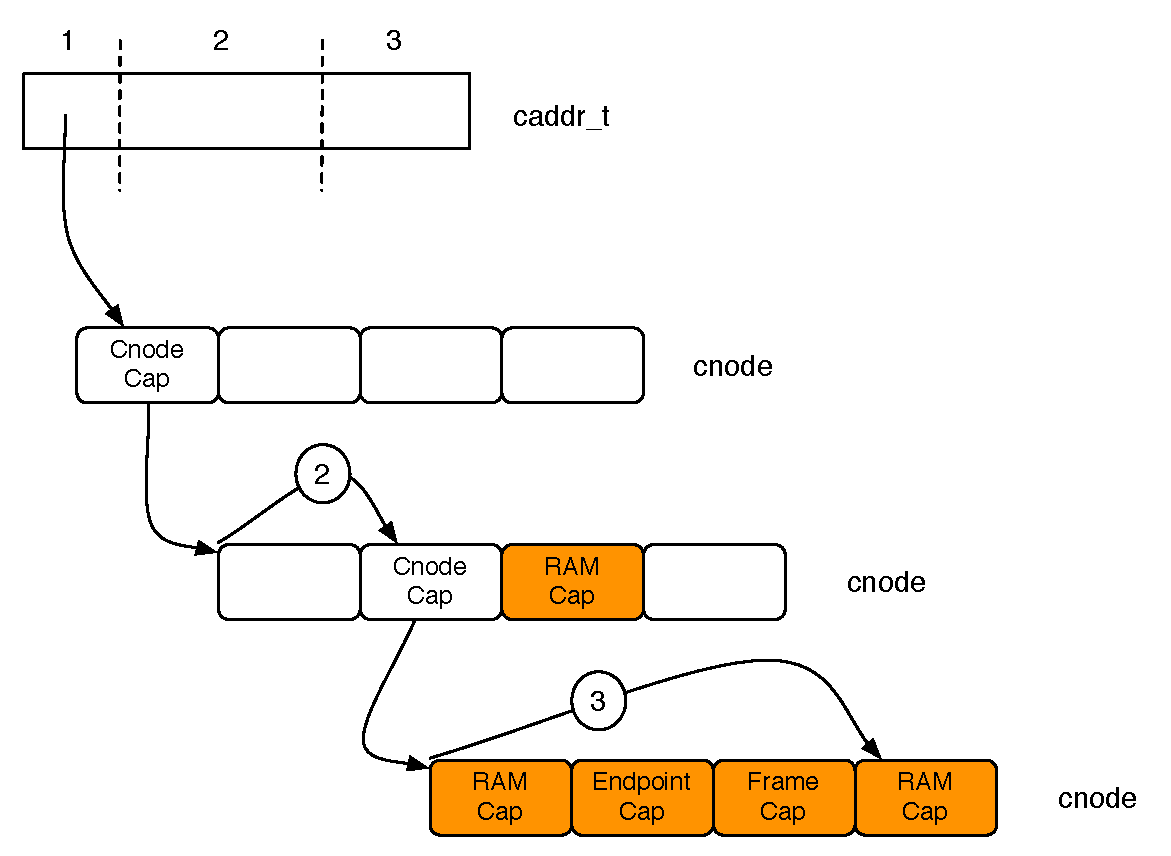
\includegraphics[width=0.4\textwidth]{cap_translation.pdf}}
  \quad
  \subfloat[Capability Hierarchy]{\label{fig:cap_hierarchy}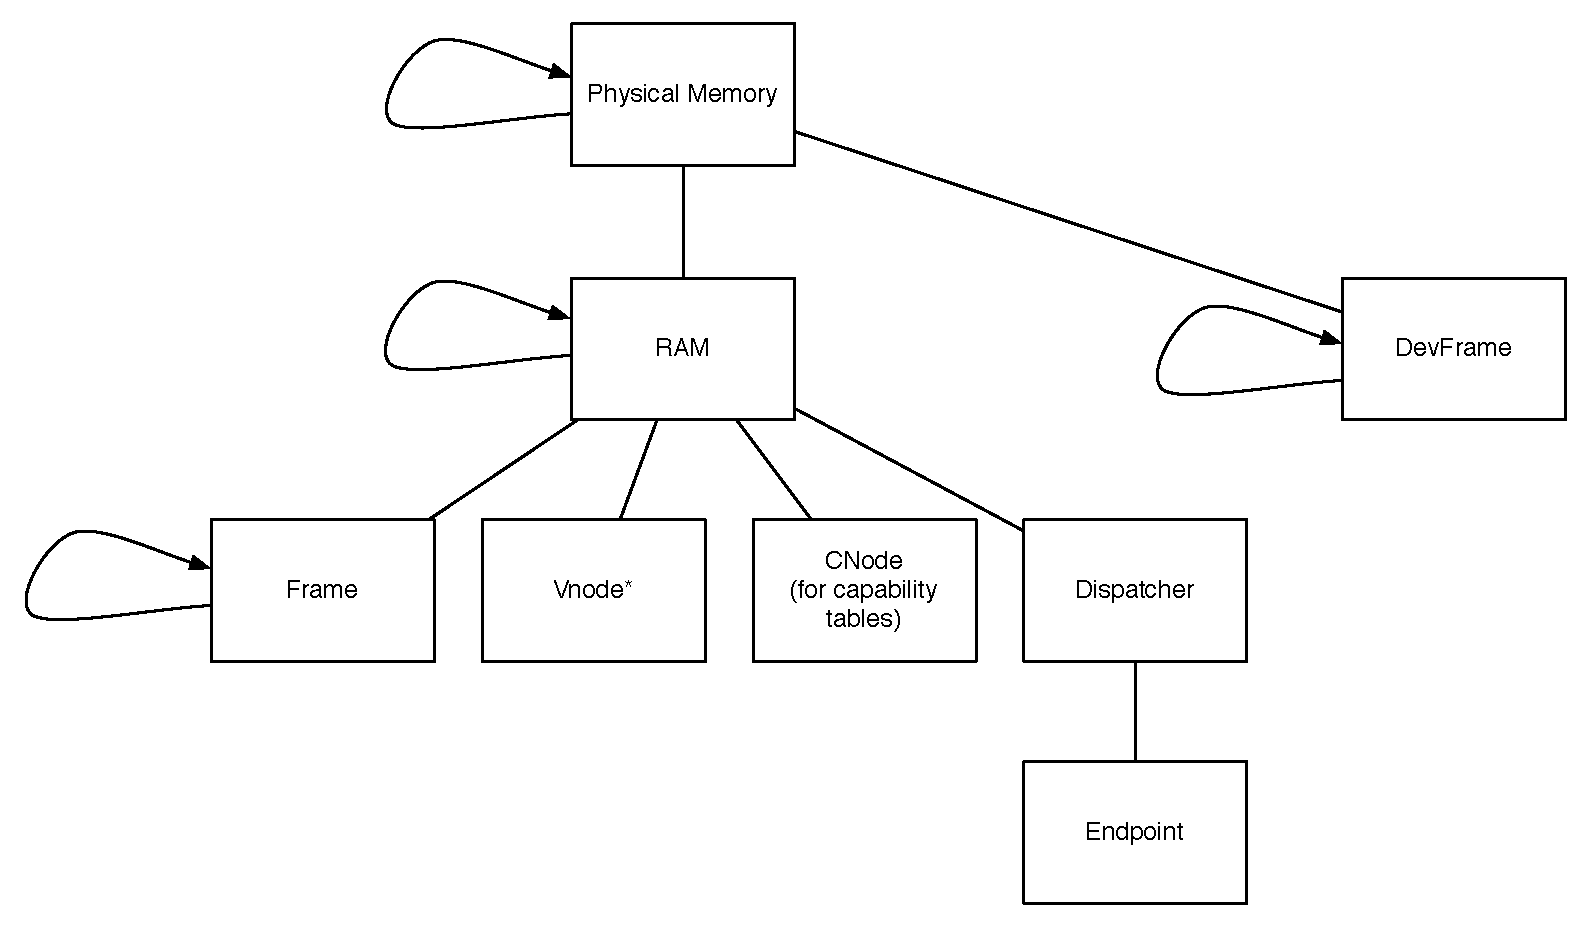
\includegraphics[width=0.5\textwidth]{cap_heirarchy.pdf}}
  \caption{Capabilities}
  \label{fig:caps}
\end{figure}

A Dispatcher only has access to the capability references in its cspace. As in
seL4, capabilities are typed, and there is a strictly defined derivation
hierarchy (e.g. Figure~\ref{fig:cap_hierarchy}).

\section{Virtual Memory}
Virtual memory in Barrelfish is similar to seL4. Frames are mapped into various
(platform specific) page table data structures to create an address
space. Shared memory is achieved by sharing Frames mapped into respective
vspaces.

\textbf{XXX: some more details needed}

\section{Monitor}
A monitor user domain runs on every core. It is special in that it is
responsible for managing the kernel data structures on that core, as well as
coordinating intra and inter core communication.

There is an communication channel between every pair of monitors running on a
system. This is set up automatically at startup time.

\textbf{XXX: some more details needed}

\section{Memory Server}
The memory server is responsible for serving RAM capabilities. It receives all
RAM capabilities at startup and distributes them to other dispatchers as
requested.

\textbf{XXX: some more details needed}

\section{Boot sequence}
Grub reads menu.lst and starts domains as specified in the file.  It first
starts the "kernel" entry, which is typically the cpu driver, on core 0. The
kernel starts init, which starts mem\_server and monitor. Monitor then starts all
entries marked with "boot", which is typically: 
\begin{itemize}
\item chips (the name server)
\item skb (system knowledge base) 
\item pci (hardware eval, as well as core enumeration, pci access, etc.)
\item boot\_manager (starts up all other domains)
\end{itemize}

When pci figures out what cores there are, then boot manager(?) starts up
kernels and monitors on all cores.

Boot manager starts up any other user domains. Extra parameters in menu.lst for
grub specify which cores the domains start on. The menu.lst info is passed to
the initial kernel by grub. The kernel passes this on to init, which passes it
on to other domains as required.



%%%%%%%%%%%%%%%%%%%%%%%%%%%%%%%%%%%%%%%%%%%%%%%%%%%%%%%%%%%%%%%%%%%%%%%%%%%%%%%%
\chapter{Source Code}\label{chap:benchmarks}

\section{Directory Structure Overview}
Files related to the material covered in this document

\begin{verbatim}

barrelfish:
kernel/dispatch.c
      include/dispatch.h

include/
    barrelfish/
        dispatch.h
        dispatcher.h
        lmp_chan.h
        lmp_endpoints.h
        ump_chan.h
        ump_endpoint.h
        ump_impl.h
        waitset.h

lib/
    barrelfish/
        lmp_chan.c
        lmp_endpoints.c
        ump_chan.c
        ump_endpoint.c
        arch/x86_64/
            dispatch.c 

if/
    myapp.if

usr/
    myapp/
        myapp.c
        Hakefile
build:
    arch/usr/myapp/_for_app_myapp/ 
        myappif_flounder_bindings.c

arch/include/if
        myappif_defs.h
        myappif_lmp_defs.h
        myappif_ump_defs.h

\end{verbatim}


\section{Writing A Sample Barrelfish Application}

Here we show how to write a simple program on Barrelfish.  \textbf{XXX:} no
error handling yet.  Refer to \texttt{usr/tests/idctest} for code with proper
error handling.

\subsection{A Simple Hello World Program}

The source for user domains is stored under \begin{verbatim}/usr\end{verbatim}. 

A simple hello world domain consists of a source file, and a Hakefile. e.g.,
\begin{verbatim}
usr/myapp
    myapp.c
    Hakefile
\end{verbatim}

For a simple hello world app, the source is trivial: a simple printf in main
will suffice (note that for output printf either uses a debug syscall to print
to the serial output, or a proper serial server if one is available).

\begin{verbatim}
#include <stdio.h> 
int main(void) {
    printf("Hello World\n");
    return 0;
}
\end{verbatim}

To build the domain, call hake.sh in the build directory. This will create a
Config.hs, Makefile, and symbolic\_targets.mk. You can add myapp in the
symbolic\_tagets, then run make to build everything. You can also explicitly ask
make to build the domain. e.g.:
\begin{verbatim}
make x86_64/sbin/myapp
\end{verbatim}

After all is built, the menu.lst needs to be modified to add the domain and have
it started. Run everything in a simulator using:

\begin{verbatim}
make sim
\end{verbatim}

\subsection{A Simple Hello World Program Using IDC}

Adding IDC (inter-dispatcher communication) is a bit more complicated. It
requires defining an interface in Flounder IDL, updating the interfaces
Hakefile, updating the domain's (myapp) Hakefile, and then adding initialization
code as well as appropriate callbacks to the source file.

An example of hello world extended with an IDC. This will run on two cores (it
can also be run on the same core), with the client dispatcher sending a message
to the server who will print out "hello message received!" when it receives the
message.


The interface consists of a single message that carries no data payload.

The server exports the interface, providing callback functions that are invoked
when the export completes, and when a client connects to the interface. After
the binding is exported it is registered with the name service so that the
client can find it. When a connection is made, and a binding created, the actual
message callback handler is registered in the binding so that whenever a message
is received on the binding it is invoked.

The client uses the name service to look up the iref of the server, then uses
this iref to bind (connect) to the server. It provides a callback that is
invoked when the bind completes. In this example the callback sends a message
over the newly formed channel.

After setting up connections, both client and server sit in a loop dispatching
incoming events (causing the appropriate callbacks to be invoked).



\textbf{myappif.if}
%\lstinputlisting{myapp/if/myappif.if}
\verbatiminput{myapp/if/myappif.if}

\textbf{myapp.c}
%\lstinputlisting{myapp/usr/myapp/myapp.c}
\verbatiminput{myapp/usr/myapp/myapp.c}

\textbf{Hakefile}
%\lstinputlisting{myapp/usr/myapp/Hakefile}
\verbatiminput{myapp/usr/myapp/Hakefile}


%%%%%%%%%%%%%%%%%%%%%%%%%%%%%%%%%%%%%%%%%%%%%%%%%%%%%%%%%%%%%%%%%%%%%%%%%%%%%%%%
\chapter{IDC: Inter Dispatcher Communication}


IDC is performed over different underlying channels, depending on the
communication mechanisms available. For example, for IDC between dispatchers on
the same core, LMP is used, while for IDC between cores, UMP (or another
mechanism depending on the architecture and what is available) is used. The
mechanism used is determined at binding time. Code for all possible bindings is
generated from the IDL descriptions.

Performing IDC involves an interface specific binding struct, a waitset, and
channels.

The binding struct is channel-type specific. It includes an appropriate channel
struct, and a channel-type independent, but interface specific, binding struct.

For example, for LMP, the channel specific binding struct is: \\
\texttt{struct myappif\_lmp\_binding (myappif\_lmp\_defs.h)}

The generic binding struct is: \texttt{struct myappif\_binding (myappif\_defs.h)}

The LMP specific channel struct is: \texttt{struct lmp\_chan in (lmp\_defs.h)}

The generic binding struct contains pointers to the sending stubs (stored in a
vtable filled in by the binder), the message handlers (provided by the client
and also stored in a vtable), and the waitset associated with the binding.

The channel struct contains all the channel-type specific data necessary to
perform the actual communication.

The waitset tracks the state of channels and threads waiting for messages
(actually events, since it also tracks things like connection events, etc.) on
those channels. It contains several queues of channel structs: the idle queue,
which stores all channels that don't have any events ready for delivery, the
pending queue, which stores the channels that have events available for
delivery, and the polled queue, which stores channels that need to be
polled. The waitset also keeps a queue of threads that are blocked waiting for
something to happen on one of the channels.

The way that channels in a waitset work is that a channel is 'triggered' when an
event occurs (or is discovered during polling) and the channel is moved to the
pending queue. Once a channel is in the pending queue, further events do not
trigger it until it has been processed and put back in the idle or polled
queues. The waitset's thread queue tracks threads that are blocked on the
waitset. Every time an event triggers a channel and causes it to be moved to the
pending queue, one thread from the waiting threads queue is unblocked, allowing
it to process a channel from the pending queue. There should never be threads in
the waiting queue if there is more than one channel in the pending queue.

see: \texttt{struct waitset (waitset.h)}

The \texttt{event\_dispatch()} function picks up the next pending channel and
returns its handler. If there are no pending channels it polls any channels on
the polled queue, triggering (and thus moving to the pending queue) any that has
an event available. If no channels have events, and there is nothing to poll
then it blocks.

Sending messages is channel-type specific.

\section{IDC\---LMP: Local Message Passing}
IDC between dispatchers on the same core uses LMP (local message passing).  LMP
uses endpoint capabilities for communication.  In this case the channel struct
contains a reference to a remote endpoint cap (for the sender) and a local
endpoint cap (for the receiver). It also contains a reference to an endpoint
structure. This is a struct contained in the receiver's dispatcher and refers to
a buffer that is used to store incoming messages. The dispatcher can have
multiple such endpoint buffers.

\begin{figure}
  \begin{center}
    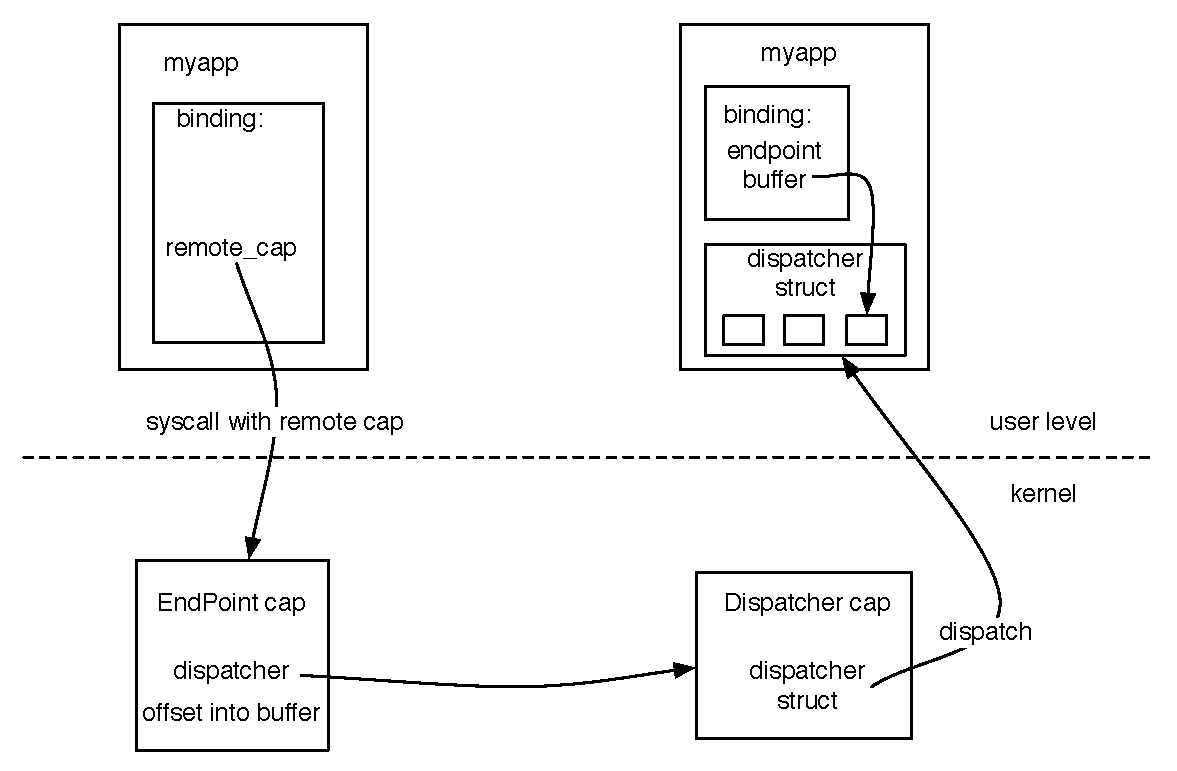
\includegraphics[width=0.5\columnwidth]{LMP.pdf}
  \end{center}
  \caption{Local Message Passing}
  \label{fig:lmp}
\end{figure}


The sender's remote endpoint cap is derived from the receiver's dispatcher cap,
and contains a pointer back to the DCB and an offset into the associated
endpoint buffer.

When a message is sent, the sender invokes the remote endpoint cap with the
message to send. This causes the kernel to copy the message into the associated
endpoint buffer and then make the receiver dispatcher runnable (which will cause
it's \texttt{run()} upcall to be invoked when it is scheduled). The run function
then finds the endpoint with a message in it and invokes the trigger on the
appropriate waitset. The channel's event handler is responsible for getting the
rest of the message out of the buffer and invoking appropriate user-defined
handlers.

Sender: \texttt{lmp\_deliver\_payload (dispatch.c)}

Receiver: \texttt{disp\_run (dispatch.c)}
          \texttt{lmp\_endpoints\_poll\_disabled (lmp\_endpoints.c)}

Event handler: \texttt{myappif\_lmp\_rx\_handler (myappif\_flounder\_bindings.c)}

\textbf{Binding:} The process of binding for LMP involves the sender creating
the endpoint capability and appropriate buffers, then invoking
\texttt{lmp\_bind\_request} on the monitor. The monitor sends the request to the
receiver, where it sets up its own endpoint cap and buffer and binding struct,
and returns the cap through the monitor to the sender.

\textbf{Passing capabilities - LMP:} When a capability is sent in a message, then
the kernel must additionally copy the cap to the receiver's cspace (a slot for
this is setup in the endpoint). The receive handler must ensure that it copies
the cap out of this cspace slot in order to free it for future transfers.

\section{IDC\---UMP: Inter-core User-level Message Passing}

IDC between dispatchers on different cores uses UMP (user-level message passing)
(on x86).

\begin{figure}
  \begin{center}
    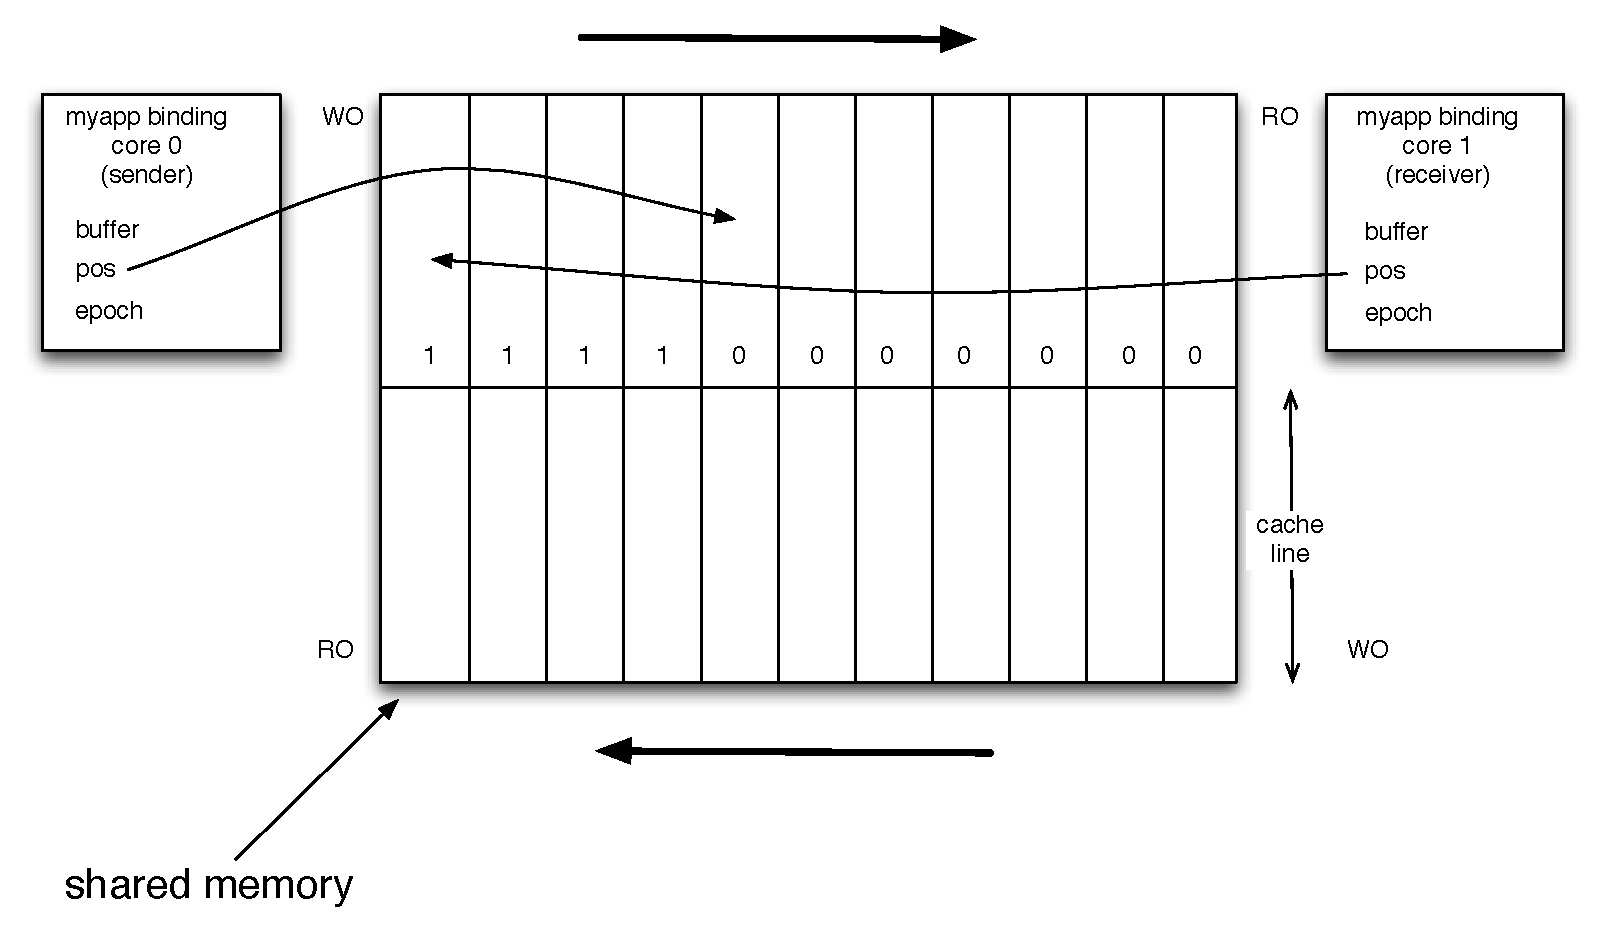
\includegraphics[width=0.5\columnwidth]{UMP.pdf}
  \end{center}
  \caption{User-level Message Passing}
  \label{fig:ump}
\end{figure}

UMP uses shared memory and polling and inter-processor interrupts for
communication. The shared memory is split into a send buffer and a receive
buffer (Figure~\ref{fig:ump}), with each entry in the buffers being the size of
a cache line. The sender writes into the send buffer, and the receiver reads
from it. The receiver polls to determine whether new messages have been
received.

The binding struct for a UMP channel contains UMP specific channel structs
(nested within various included structs) which contain a reference to the shared
memory, as well as a counter specifying the current read or write position.

In order to detect whether the write position has been reached when reading, the
channel also contains an epoch flag. Every buffer entry has an epoch bit that is
flipped every time a new entry is added. When reading a new entry the channels's
epoch is compared to the epoch bit of the buffer slot to be read. If it is the
same, then the entry is valid, if it is different then it is not valid. The
channel's epoch flag is flipped every time the counter wraps around.

The sender also has to know whether it is going to run up against the
receivers's read position. Rather than flip epoch bits on a read (in order to
avoid bouncing cache lines the buffer is kept write-only for the sender and
read-only for the receiver) each message has a sequence id. When replying to the
sender the receiver sends its latest read sequence id. The sender then knows how
many messages are outstanding and together with knowledge of the buffer size,
can avoid overwriting messages that haven't been read yet.

\textbf{Binding:} The UMP binding process involves the source creating the
channel buffers, then sending a cap to the buffer along with a bind request
through LMP to the monitor. The monitor serialises the cap and sends it through
to the destination monitor. The destination monitor recreates the cap, and sends
it on to the receiver. This sets up its channel struct accordingly and finalises
the binding.

\textbf{Passing capabilities - UMP:} UMP messages containing capabilities must
be sent in two phases. The non-cap message is sent as normal. The capability
must be sent through the monitor as only the monitor is able to invoke a syscall
to serialise and deserialise a capability. The sender sends the capability with
a request to the monitor, the monitor serialises it and sends it to the
destination monitor, where it is deserialised, and send through LMP to the
destination.



%%%%%%%%%%%%%%%%%%%%%%%%%%%%%%%%%%%%%%%%%%%%%%%%%%%%%%%%%%%%%%%%%%%%%%%%%%%%%%%%
\bibliographystyle{abbrvnat}
\bibliography{paper}

\end{document}
